\documentclass[a4paper]{article}
\usepackage[english]{babel}
\usepackage[utf8]{inputenc}
% package for including graphics with figure-environment
\usepackage{verbatim}
\usepackage{graphicx}
\usepackage{hyperref}
\usepackage{float}
% colors for hyperlinks
% colored borders (false) colored text (true)
\hypersetup{colorlinks=true,citecolor=black,filecolor=black,linkcolor=black,urlcolor=black}

% package for bibliography
\usepackage[authoryear,round]{natbib}
% package for header
\usepackage[automark]{scrpage2}
\pagestyle{scrheadings}
\ihead[]{Andreas Gerlach}
\ohead[]{\today}
\cfoot[]{\pagemark}
\setheadsepline[122mm]{0.3mm}
\begin{document}
	\title{
	\begin{figure}[!ht]
		\flushleft
			
\includegraphics[width=0.7\textwidth]{logo.eps}
	\end{figure}
	\vspace{1cm}
	\begin{figure}[!ht]
	    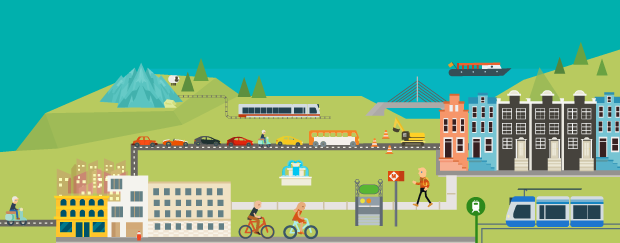
\includegraphics[width=\textwidth]{Connected_commuters_SSpage.png}
	\end{figure}
	\vspace{1cm}
	\Huge The Easy Way \\
	}

	\vspace{1cm}

	% if you are the only author, you might use the following
	% \author{Name of student}

	% Insert here your name and correct mail address
	\author{\Large \href{mailto:andreas.gerlach@smail.fh-koeln.de}{Andreas Gerlach}
	\vspace{1cm}}

	% name of the course and module
	\date{
	\large Module: Foundations and Principles II \\ Course: eEntrepreneurship \\
	\vspace{0.8cm}
	\large Lecturer: William Sen \\
	\vspace{1cm}
	\today
	}

	\maketitle
	\setlength{\parindent}{0pt}

	\newpage
	\tableofcontents
	\newpage
	\listoffigures
	\vspace{2cm}
	\listoftables
	\newpage

\section{Introduction} % (fold)
\label{sec:introduction}

\textit{The Easy Way} is a new online service that provides guidance and support for planning your trip via public transportation services. Beside being able to search for a connection between starting point and your destination for the expected date and time of the trip it will also give you real­time feedback on the day of travel related to delays or possible connections you might not be able to reach. In the latter case it will also give you instant alternatives that you could take for getting to your destination including the expected overall delay of arrival. If there is an intermediate stop on your track and you will have to wait a certain amount of time for your connection it shows you personalised offers that you can use for spending the time on the intermediate location. These offers  can  include  bars, restaurants, shops, museums, historical buildings as well as other sightseeings.  It  can  be  combined  with  promotional  offers  from the respective owner of the location and includes the distance from the station and the time that you have left to spend there as  well.  For  sure  when  accepting  such  an  offer  the  service  will  also  inform you via push notification  when  it’s  time  to  leave  to get the connection train or bus based on the current situation. \par \vspace{0.2cm}
If you travel a lot --­ let’s say during your daily commute --­ it might be interesting to see if other people you know might be nearby your travel route so that you can arrange an appointment -- for let’s say a dinner or so. Therefore \textit{The Easy Way} service can be connected to your social network profiles (e.g. Facebook, Twitter, Google+) so that it knows your relatives and can offer you possible matches. If you want to arrange a meeting at a specific location with one or more relatives you can do so right from within the service, that will on your behalf utilise the corresponding social network service API to send a post to your selected friends and followers.

\subsection{Vision}
\label{subsec:vision}

The vision behind \textit{The Easy Way} is: ''make commuting and travelling with public transportation services an enjoyable and straightforward experience".

\subsection{Key aspects}
\label{subsec:aspects}

The \textbf{key aspects} that the service wants to address are:

\begin{enumerate}
\item easily plan your trip with public transportation service in a sophisticated online or mobile application
\item  get instantaneous feedback to your trip via push notifications on your smartphone that might include delays or connection you will not reach (based on current traffic situation)
\item  rearrange your connection based on proposals of the application and check your expected overall delay of arrival
\item  get promotional offers for points of interest on your track or intermediate stop locations
\item  arrange an ad­hoc appointment with friends and followers
\end{enumerate}

\subsection{Key Questions}
\label{subsec:questions}

The following open issues have to be clarified upfront and can be likely solved with the information provided by the sources listed here:

\begin{table}[ht]
\begin{tabular}{|p{0.60\textwidth}|p{0.40\textwidth}|}
\hline
\textbf{Topic} & \textbf{Sources} \\
\hline
     How to query and combine information from different public transportation services (e.g. Deutsche Bahn, BVG, …)?   &  http://www.bahn.de, http://www.bvg.de, … \\
\hline
     Check conditions of cloud infrastructure provider (e.g. Amazon, Google, Microsoft).
    & http://aws.amazon.com, https://cloud.google.com, ... \\
\hline
     Check available online advertising providers and their conditions (e.g. Google AdSense, Google AdWords).
    & https://www.google.com/ adsense, https://www.google.com/ adwords \\
\hline
     Build up a database with points of interest and set up partnerships with their owners.
    & https://www.google.de, http://www.berlin.de, http://www.koeln.de, … \\
\hline
     Find first-­movers to try out the service and use them to advertise it later .
    & http://www.twitter.com, http://www.facebook.com, … \\
\hline
    Find investors and business partners to build first version of the platform and it's mobile applications.
    & http://www.kickstarter.com, http://www.indigogo.com, ... \\
\hline
\end{tabular}
\caption{Information Retrieval Sources}
\label{tab:inforetrieval}
\end{table}

\subsection{Revenue Streams}
\label{subsec:revenue}

The service is offered for free for end-users. They can register to it via the web site or by using one of the mobile applications. An important revenue stream for the service will be the monthly fee that business customers have to pay to participate on the platform and offer their products and services on it. Anonymous user information will be made available for analysing the success of those advertisings. Additionally the mobile applications will include mobile advertising as well as an in-app purchase option to get rid of them.

% section introduction (end)

\section{Objectives}
\label{sec:objectives}

The first 3 major objectives, that \textit{The Easy Way} will address, are as follows:

\begin{enumerate}
\item integrate at least 5 major cities w/ local transportation, sightseeings and other points of interest
\item  get into the TOP 20 for travelling applications in the mobile application stores from Apple (AppStore), Google (Play Store) and Microsoft (Windows Store)
\item  get a turnover of 10 000 EUR per month from advertising partners on the platform
\end{enumerate}

\section{Distribution and Sales Channels} % (fold)
\label{sec:channels}

\subsection{Offline Channels}

As our service relies on objects in the real-world -- like bars, restaurants, stations, time-tables, we will have to place links to our online service on those real-world objects. This will allow us to get in touch with people just arriving at or ''using" those real-world objects. We will focus on ease-of-use and the value-added service our product promise to them. This will likely get them interested to try out our service the next time.

\begin{itemize}

\item   Place billboards on main stations saying ''Welcome to … Please scan the QR code to get information about points of interest and special offers!". If end user scans the QR code with his smartphone or tablet he will be routed to a mobile landing page that will include links to the native apps in the App Stores as well as provide registration and user profile maintenance functionality. This one will increase the penetration of the platform and the mobile applications (objective 2, 3).

\item  Actively participate on important exhibitions --­ e.g. ITB Berlin, to help build a network of partners who works or are attached to the platform (objective 1, 3).

\item  Print flyers and distribute them through bars, restaurants, tourist info offices, travel agencies (objective 1, 2, 3).

\item  Create postal cards with funny pictures and slogans that will be placed in bars or restaurants --­ e.g. edgar freecards (objective 2, 3).

\item  Write an article or prepare an interview to be published into a travel agent magazine --­ e.g. customer magazine of Deutsche Bahn (objective 2, 3).

\item  Provide funny accessories like t-­shirts, notebook stickers, bags, … to the early adopters so that they can spread the message of your service (objective 2, 3).

\end{itemize}

\subsection{Online Channels}

As our service is a Web-based product we can make use of the full range of marketing and distribution channels that the Internet provides for us. In addition to that we can also provide our first-movers and customers with the possibility to promote our service to their friends and followers via the Social networks.

\begin{itemize}

\item  Use social media to communicate the benefits of the service to a wider audience. This could affect end users and partners alike. Set up an own blog, Twitter, Facebook and Google+ channel, write about success stories and user experiences in case studies and track user feedback on each platform (objective 2, 3).

\item  Promoting the smartphone apps on the respective stores by doing special pricing, participating on ''App of the week" or getting an official recommendation of the app store owner (objective 2).

\item  Provide an user community feature on the web page to let users queue in bugs and feature requests for the application and service. Let the users vote for most important features, missing points­of­interest, bars, restaurants, …. and inform them when you plan to integrate those (objective 1, 2).

\item Set up a bonus system that will give an existing partner a gratification for advertising a new member to the platform (objective 1, 3).

\item  Use Google AdWords to place online advertising on search results that either deals with specific locations that are available on the service or when looking up travel routes in general (objective 1, 3).

\item  Create an YouTube channel and host short video clips that explains the service and success stories (Simple Show style) for communicating the user stories visually (objective 1, 2, 3).

\end{itemize}

% section foundations (end)

\section{Customer Groups} % (fold)
\label{sec:segmentation}

At first we would focus on early adopters of the platform, which are likely jumping onto the service for its features and could be used to publish success stories on our site to address an even wider audience later. Those first early adopters would include:

\begin{enumerate}
\item  Business Travellers
\item  Daily Commuters
\item  City Travellers
\item  Business Owners
\end{enumerate}

\textbf{Business Travellers} are possibly interested in the platform as they are travelling around the country a lot, might have some spare time on stations or the airport, or are even staying at an unfamiliar destination location for some time. \par \vspace{0.2cm}
\textbf{Daily Commuters} travelling the same route twice every day: first from home to work, later in the opposite direction. Although they will know the route inside-­out they will likely face traffic jam, will miss connection trains or buses and have to stay some time on an intermediate station of the route. Additionally they are likely participating in arranging appointments with relatives or friends based on their current time schedule and possible crossing points with them. \par \vspace{0.2cm}
\textbf{City Travellers} are hopping to a city for a short time-frame like a weekend or so as part of a vacation. They will either go to a city they have never been before or plan the trip to a known location to meet some friends. In both situations they might be interested in the platform to find interesting locations for their next city trip. \par \vspace{0.2cm}
\textbf{Business Owners} can use the platform to advertise special offers to these aforementioned groups of people to get them interested in visiting their store or shop. This would give them a targeted communication channel to reach them and their specific needs.

% section methodology (end)

\section{Lead Generation} % (fold)
\label{sec:lead}

A lead generation is a way to uniquely communicate with potential customers to get them interested in our products and services and address their specific needs, so that they will get attached to our business and are more likely to buy from us at the end.

\begin{figure}[!ht]
    \center
        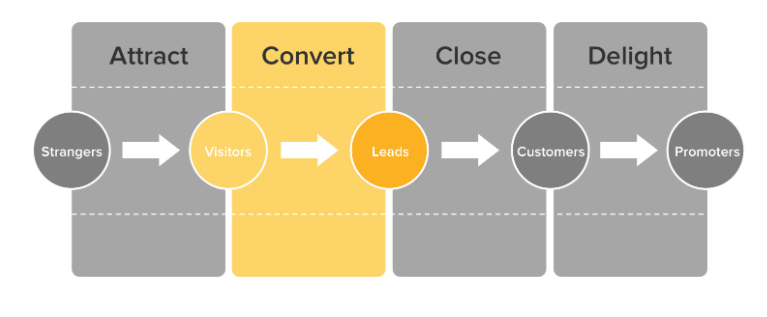
\includegraphics[width=\textwidth]{From_Strangers_to_Promoters.png}
    \caption{Lead Generation Process}
    \label{fig:leadgen}
\end{figure}

As said, the lead generation process has to uniquely address the needs of our customers / customer groups. That also means we will have to set up different lead generation processes for our target groups mentioned above. \par \vspace{0.2cm}
Travellers and Commuters (B2C) can be addressed via a \textbf{landing page} that will provide them with  the  possibility  to  download  the  required  mobile  apps  (via  links  to  the  corresponding AppStore) as well as \textbf{subscribe to our monthly newsletter}, that holds information about new locations attached to the platform, showing \textbf{user success stories} as well as offering special promotional coupon codes. Links to this landing page can be placed on our billboards at the stations, on our flyers at the restaurants and bars or on our free postal cards in form of a machine readable QR code, promoted via Social Networks like Facebook and Twitter as well as part of our advertising we place  in a form of \textbf{Call­to­Action messages} via Google AdWords. The latter ones could be displayed on travel planning sites on the Internet as well (e.g. www.bahn.de). Existing customers will be interviewed and the experience will be shared on our web site in textual format or as YouTube video story, offering a Call­to­Action to join the platform. Those stories  will  also  be  announced  via  Social  Media  channels.  All  actions  on  the Social Media channels will be monitored and repeated after a certain amount of time. \par \vspace{0.2cm}
Business Owners (B2B) will be likely a little bit harder to convince to join the platform. We will present them with some \textbf{success stories and interviews} of early adopters (customers and business owners) as well as provide \textbf{successful case studies} of business owners that shows some  figures about increase of number of customers, higher customer satisfaction and business turnover. Those can be accessed freely on our web site and we provide a Call­to­Action to get an \textbf{introductory offer} for the first 30 days of joining the platform by filling out an email form. For business customers we would also offer to include their business success story in our monthly newsletter or post about it on our Social Media channels, which allows them to advertise their brand via our communication channels. This could also attract new customers to join the platform and have their business addressed as well. \par \vspace{0.2cm}
Having our lead generation process on the Internet will be the most cost-­effective solution as we have nearly zero effort to put the landing page on our web servers and distribute the links to them via our Social Media channels. We will have to spend money continuously on the billboards (design,  print  and  placement) and therefore will monitor the conversion rate of this channel regularly. We will also need some resources (money, personal) to prepare and make the interviews with potential and existing customers (B2B, B2C) and finalise them later so they can be placed online or in the newsletter as well. The same is true for setting up the monthly newsletter. We might use students in the beginning for those working packages to save some money. As the amount we have to spend to Google AdWords depends on the keywords we register for and the number of clicks we receive, it could also consume a lot of money (especially as the travel industry is an huge market with lot of businesses fighting for customer attention the amount we have to spend for the keywords would rather be high than low). We are therefore monitoring the conversion rate from that channel continuously as well. The introductory offer for the newcomers in the business sphere might effectively also cost us nearly nothing, we already invest in the IT infrastructure and software so that hosting some offers of the business for the first 30 days might (only) consume resources that are already in place.

% section results (end)

\end{document}
